 \documentclass{beamer}[10]

\usepackage{graphicx}
\usepackage{xcolor}
\usepackage{tabto}
%\usepackage{beamerthemesplit}
\usepackage{tikz}
\usepackage{cancel}
\usepackage{verbatim}
\usepackage{fancybox}
\usepackage{enumerate}
\usepackage{amsmath,amssymb,amsthm,textcomp,mathtools}
\usepackage[super]{nth}
\usepackage[amssymb]{SIunits}
\usepackage{booktabs}
\usepackage{cancel}
\usepackage{bm}
\usepackage[utf8]{inputenc}
\usepackage{tabularx}
\usepackage{ragged2e}
\newcolumntype{Y}{ >{\RaggedRight\arraybackslash}X}
\usetikzlibrary{arrows,shapes}
\newcommand\T{\rule{0pt}{2.6ex}}
\newcommand\B{\rule[-1.2ex]{0pt}{0pt}}
\definecolor{UUcrimson}{RGB}{204,0,0}
\mode<presentation>
{ \usetheme{default}
  \usecolortheme[named=UUcrimson]{structure}
  \useinnertheme{circles}
  \setbeamercovered{transparent}
  \setbeamertemplate{blocks}[rounded]
  \usefonttheme[onlymath]{serif}
  \setbeamertemplate{navigation symbols}{}
  \setbeamertemplate{footline}[page number]
  \setbeamertemplate{navigation symbols}{}
  \setbeamercolor{section in toc}{fg=black,bg=white}
  \setbeamercolor{alerted text}{fg=UUcrimson!80!gray}
  \setbeamercolor*{palette primary}{fg=white,bg=UUcrimson}
  \setbeamercolor*{palette secondary}{fg=UUcrimson!70!black,bg=gray!15!white}
  \setbeamercolor*{palette tertiary}{bg=UUcrimson!80!black,fg=gray!10!white}
  \setbeamercolor*{palette quaternary}{fg=UUcrimson,bg=gray!5!white}
  \setbeamercolor*{palette sidebar primary}{fg=UUcrimson!10!black}
  \setbeamercolor*{palette sidebar secondary}{fg=white}
  \setbeamercolor*{palette sidebar tertiary}{fg=UUcrimson!50!black}
  \setbeamercolor*{palette sidebar quaternary}{fg=gray!10!white}
  \setbeamercolor{titlelike}{parent=palette primary,fg=white}
  \setbeamercolor{frametitle}{bg=UUcrimson}
  \setbeamercolor{frametitle right}{bg=UUcrimson}
  \setbeamercolor*{separation line}{}
  \setbeamercolor*{fine separation line}{}
}

\usetikzlibrary{backgrounds}
\makeatletter
\tikzstyle{every picture}+=[remember picture]
\tikzset{%
  fancy quotes/.style={
    text width=\fq@width pt,
    align=justify,
    inner sep=1em,
    anchor=north west,
    minimum width=\linewidth,
    font=\itshape
  },
  fancy quotes width/.initial={.8\linewidth},
  fancy quotes marks/.style={
    scale=8,
    text=white,
    inner sep=0pt,
  },
  fancy quotes opening/.style={
    fancy quotes marks,
  },
  fancy quotes closing/.style={
    fancy quotes marks,
  },
  fancy quotes background/.style={
    show background rectangle,
    inner frame xsep=0pt,
    background rectangle/.style={
      fill=gray!25,
      rounded corners,
    },
  }
}
\newenvironment{fancyquotes}[1][]{%
\noindent
\tikzpicture[fancy quotes background]
\node[fancy quotes opening,anchor=north west] (fq@ul) at (0,0) {``};
\tikz@scan@one@point\pgfutil@firstofone(fq@ul.east)
\pgfmathsetmacro{\fq@width}{\linewidth - 2*\pgf@x}
\node[fancy quotes,#1] (fq@txt) at (fq@ul.north west) \bgroup}
{\egroup;
\node[overlay,fancy quotes closing,anchor=east] at (fq@txt.south east) {''};
\endtikzpicture}
\makeatother

\usepackage{scalerel}[2014/03/10]
\usepackage{stackengine}
\usepackage{empheq}
\newcommand*\widefbox[1]{\fbox{\hspace{0.5em}#1\hspace{0.5em}}}

\newcommand\reallywidetilde[1]{\ThisStyle{%
  \setbox0=\hbox{$\SavedStyle#1$}%
  \stackengine{-.1\LMpt}{$\SavedStyle#1$}{%
    \stretchto{\scaleto{\SavedStyle\mkern.2mu\sim}{.5467\wd0}}{.4\ht0}%
%    .2mu is the kern imbalance when clipping white space
%    .5467++++ is \ht/[kerned \wd] aspect ratio for \sim glyph
  }{O}{c}{F}{T}{S}%
}}
\usepackage{media9}

\logo{
\includegraphics[width=0.75cm]{logo.jpg}}
\author[Gibbs]{Dr. Jeremy A. Gibbs}
\institute{Department of Mechanical Engineering\\University of Utah}
\date{Fall 2016}
\title{LES of Turbulent Flows: Lecture 16}
\begin{document}

%----------------------------------------------------------------------------------------
%	TITLE & TOC SLIDES
%----------------------------------------------------------------------------------------

\begin{frame} 
  \titlepage
\end{frame}

%------------------------------------------------

\begin{frame}
\frametitle{Overview}
\tableofcontents
\end{frame}

%------------------------------------------------
\section{Mixed Models} %
%------------------------------------------------
\begin{frame}{Mixed Models}
\begin{itemize}
	\item Both the similarity and nonlinear models exhibit a high level of correlation in \textit{a priori} tests with measured values of $\tau_{ij}^{\Delta}$, but they underestimate the average dissipation and are numerically unstable
	\item Typically they are combined with an eddy-viscosity model to provide the proper level of dissipation.
\end{itemize}

\end{frame}

%------------------------------------------------
\begin{frame}{Mixed Models}
\begin{itemize}
	\item An example is (Bardina et al. 1980)
	$$\boxed{\tau_{ij} = C_L \left( \overline{\widetilde{u}_i\widetilde{u}_j} - \overline{\widetilde{u}_i}\; \overline{\widetilde{u}_j} \right) - 2(C_S \Delta)^2|\widetilde{S}|\widetilde{S}_{ij}}$$
	\item The similarity term has a high level of correlation with $\tau_{ij}^{\Delta}$ and the eddy-viscosity term provides the appropriate level of dissipation.
\end{itemize}

\end{frame}

%------------------------------------------------
\begin{frame}{Mixed Models}
\begin{itemize}
	\item Proper justification for the mixed model did not exist at first but a more unified theory has developed in the form of approximate deconvolution or filter reconstruction modeling (Guerts pg 200, Sagaut pg 210)
	\item Idea: a SGS model should be built from 2 parts
\end{itemize}

\end{frame}

%------------------------------------------------
\begin{frame}{Mixed Models}
\begin{columns}[T]
    \begin{column}{.55\textwidth}
    \begin{minipage}[c][.6\textheight][c]{\linewidth}
    \begin{itemize}
	\item The \textbf{first part} accounts for the effect of the filter through an approximate reconstruction of the filter’s effect on the velocity field (note the similarity model is a zero-order filter reconstruction). 
	\item This is the model for the resolved SFS.
\end{itemize}
      \end{minipage}
    \end{column}
    \begin{column}{.55\textwidth}
      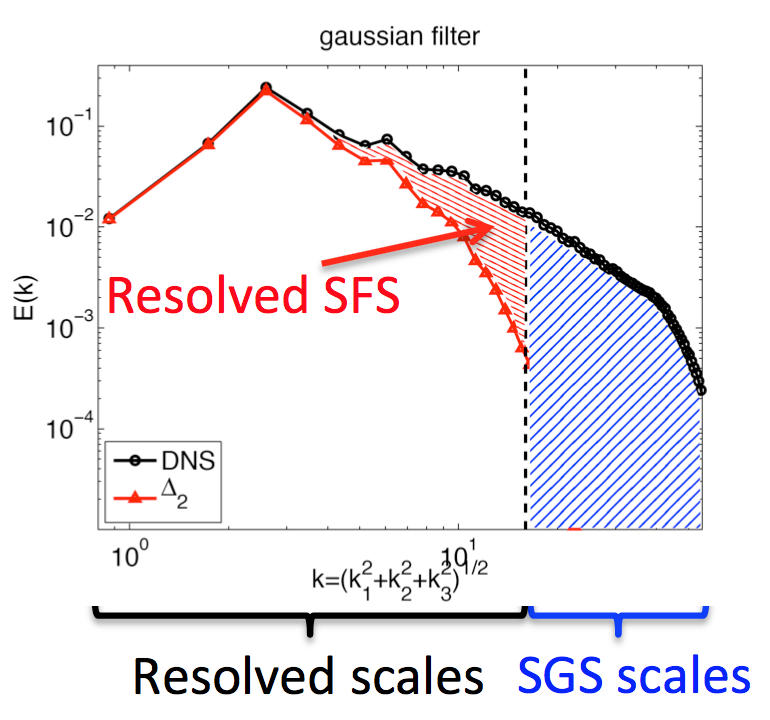
\includegraphics[width=\textwidth]{sfs}
    \end{column}
  \end{columns}
\end{frame}
%------------------------------------------------
\begin{frame}{Mixed Models}
\begin{columns}[T]
    \begin{column}{.55\textwidth}
    \begin{minipage}[c][.6\textheight][c]{\linewidth}
    \begin{itemize}
	\item The \textbf{second part} accounts for the SGS component of $\tau_{ij}$
	\item We then assume that we can build $\tau_{ij}$ as a linear combination of these two model components.
\end{itemize}
      \end{minipage}
    \end{column}
    \begin{column}{.55\textwidth}
      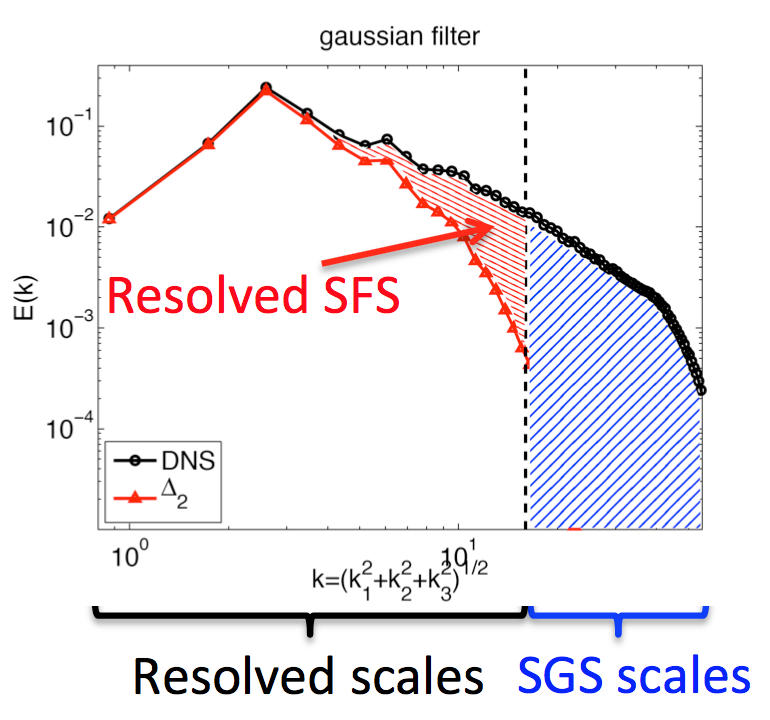
\includegraphics[width=\textwidth]{sfs}
    \end{column}
  \end{columns}
\end{frame}

%------------------------------------------------
\begin{frame}{Mixed Models}
A few last notes on Similarity models
    \begin{itemize}
	\item Bardina's model is exactly zero for a spectral cutoff filter
	\item Liu et al. form of the similarity model also fails. This is credited to the nonlocal structure of the cutoff filter. It breaks the central assumption of the similarity model -- that the locally $\tau_{ij}$ decomposed at different levels is self similar
\end{itemize}
\end{frame}

%------------------------------------------------
\begin{frame}{Modulated Gradient Model}
    \begin{itemize}
	\item A related model of similar form to the nonlinear model is the Modulated Gradient Model (see Lu et al. 2008 and Lu and Port\'{e}-Agel 2010)
	\item The goal is to improve the magnitude of the $\tau_{ij}$ estimates while keeping the high level of correlation observed for nonlinear (gradient) models
\end{itemize}
\end{frame}

%------------------------------------------------
\begin{frame}{Modulated Gradient Model}
    \begin{itemize}
	\item Assume
	$$\tau_{ij} = \widetilde{k}_r C_{ij}$$
	where for consistency $C_{kk} = 2$
	\item Using our resolved stress $L_{ij} = \overline{\widetilde{u}_i\widetilde{u}_j} - \overline{\widetilde{u}_i}\; \overline{\widetilde{u}_j}$ and the Germano identity (more later), we can show that approximately
	$$C_{ij} = 2(L_{ij}/L_{kk}) \Rightarrow \tau_{ij} = 2\widetilde{k}_r(L_{ij}/L_{kk})$$
\end{itemize}
\end{frame}

%------------------------------------------------
\begin{frame}{Modulated Gradient Model}
    \begin{itemize}
	\item This model suffers from some drawbacks, such as  insufficient dissipation at high Re and that it is not material frame indifferent
	\item The authors suggested an improvement by replacing $L_{ij}$ with $\widetilde{A}_{ik}$
	$$\tau_{ij} = 2\widetilde{k}_r (\widetilde{A}_{ij} \widetilde{A}_{kk})$$
	Note: we can also use
	$$\widetilde{G}_{ij} = \frac{\Delta_x^2}{12}\frac{\partial \widetilde{u}_i}{\partial x}\frac{\partial \widetilde{u}_j}{\partial x} + \frac{\Delta_y^2}{12}\frac{\partial \widetilde{u}_i}{\partial y}\frac{\partial \widetilde{u}_j}{\partial y} + \frac{\Delta_z^2}{12}\frac{\partial \widetilde{u}_i}{\partial z}\frac{\partial \widetilde{u}_j}{\partial z}$$
\end{itemize}
\end{frame}

%------------------------------------------------
\section{Dynamic SGS Models} %
%------------------------------------------------
\begin{frame}{Dynamic SGS Models}
\begin{itemize}
	\item So far we have given a general description of some commonly used SGS models
	\item \textbf{All of these models include at least one model coefficient} that must be prescribed, either based on theory with a specific set of assumptions (usually isotropy), from experimental data, or chosen ad hoc to get the ``correct'' \textit{a posteriori} results from simulations
	\item  Germano et al. (1991) developed a procedure to dynamically calculate these unknown model coefficients
	\item For scalars and compressible flow see Moin et al., PofF, (1991)
\end{itemize}

\end{frame}

%------------------------------------------------
\begin{frame}{Dynamic SGS Models}
\begin{itemize}
	\item  Recall: applying a low-pass filter to the N-S equations with a filter of characteristic width $\Delta$ (denoted by $\widetilde{\ \ }$) results in the unknown SFS stress term:
	\begin{equation}
	\label{sfs1}
	\boxed{\tau_{ij} = \widetilde{u_iu_j} - \widetilde{u}_i \widetilde{u}_j}
	\end{equation}
	\item This term must be modeled with an SGS model to close our equation set
\end{itemize}

\end{frame}

%------------------------------------------------
\begin{frame}{Dynamic SGS Models}
\begin{itemize}
	\item   We can apply another filter (referred to as a test filter) to the filtered N-S equations at a larger scale (say $2\Delta$) denoted by a bar (-):
	$$\overline{\frac{\partial \widetilde{u}_i}{\partial t}} + \overline{\frac{\partial \widetilde{u}_i \widetilde{u}_j}{\partial x_j}} = - \overline{\frac{\partial \widetilde{p}}{\partial x_i}} + \overline{\frac{1}{\text{Re}}\frac{\partial^2\widetilde{u}_i}{\partial x_j^2}} - \overline{\frac{\partial \tau_{ij}}{\partial x_j}} + F_i$$
	\item Our LES filter properties (commutation with differentiation) allows us to rewrite in standard filtered form
	$$\frac{\partial \overline{\widetilde{u}_i}}{\partial t} + \frac{\partial \overline{\widetilde{u}_i \widetilde{u}_j}}{\partial x_j} = - \frac{\partial \overline{\widetilde{p}}}{\partial x_i} + \frac{1}{\text{Re}}\frac{\partial^2\overline{\widetilde{u}_i}}{\partial x_j^2} - \frac{\partial \overline{\tau}_{ij}}{\partial x_j} + F_i$$
\end{itemize}

\end{frame}

%------------------------------------------------
\begin{frame}{Dynamic SGS Models}
\begin{itemize}
	\item The convective term can be reformatted into our standard format using the same method we used for the original filtered LES equations (see Lecture 6)
	\begin{align*}
	\frac{\partial \overline{\widetilde{u}_i \widetilde{u}_j}}{\partial x_j} &= \frac{\partial}{\partial x_j}\left(\overline{\widetilde{u}_i \widetilde{u}_j} - \overline{\widetilde{u}_i}\;\overline{\widetilde{u}_j} + \overline{\widetilde{u}_i}\;\overline{\widetilde{u}_j}\right)\\&= \underbrace{\frac{\partial \overline{\widetilde{u}_i}\;\overline{\widetilde{u}_j}}{\partial x_j}}_{\text{I}} + \underbrace{\frac{\partial \left(\overline{\widetilde{u}_i \widetilde{u}_j} - \overline{\widetilde{u}_i}\; \overline{\widetilde{u}_j}\right)}{\partial x_j}}_{\text{II}}
	\end{align*}
	\item Term I is our standard form and we can move Term II to the RHS of our expression
\end{itemize}

\end{frame}

%------------------------------------------------
\begin{frame}{Dynamic SGS Models}
\begin{itemize}
	\item Rearranging yields
	\begin{align*}
	\frac{\partial \overline{\widetilde{u}_i}}{\partial t} + \frac{\partial \overline{\widetilde{u}_i}\;\overline{\widetilde{u}_j}}{\partial x_j} = &- \frac{\partial \overline{\widetilde{p}}}{\partial x_i} + \frac{1}{\text{Re}}\frac{\partial^2\overline{\widetilde{u}_i}}{\partial x_j^2}\\&- \frac{\partial \overline{\tau}_{ij}}{\partial x_j} - \frac{\partial \left(\overline{\widetilde{u}_i \widetilde{u}_j} - \overline{\widetilde{u}_i}\; \overline{\widetilde{u}_j}\right)}{\partial x_j}+ F_i
	\end{align*}
	Note: $\overline{\tau_{ij}} = \overline{\widetilde{u_i u_j}} - \overline{\widetilde{u}_i\widetilde{u}_j}$
	\begin{align*}
	\frac{\partial \overline{\widetilde{u}_i}}{\partial t} + \frac{\partial \overline{\widetilde{u}_i}\;\overline{\widetilde{u}_j}}{\partial x_j} = &- \frac{\partial \overline{\widetilde{p}}}{\partial x_i} + \frac{1}{\text{Re}}\frac{\partial^2\overline{\widetilde{u}_i}}{\partial x_j^2}\\&- \frac{\partial \left( \overline{\widetilde{u_i u_j}} - \cancelto{}{\overline{\widetilde{u}_i\widetilde{u}_j}}- \cancelto{}{\overline{\widetilde{u}_i \widetilde{u}_j}} + \overline{\widetilde{u}_i}\; \overline{\widetilde{u}_j}\right)}{\partial x_j}+ F_i
	\end{align*}
\end{itemize}

\end{frame}

%------------------------------------------------
\begin{frame}{Dynamic SGS Models}
\begin{itemize}
	\item We can now write the SFS stress at the $2\Delta$ level as:
	\begin{equation}
	\label{sfs2}
	\boxed{T_{ij} = \overline{\widetilde{u_i u_j}} - \overline{\widetilde{u}_i}\; \overline{\widetilde{u}_j}}
	\end{equation}
	which leads to 
	$$\frac{\partial \overline{\widetilde{u}_i}}{\partial t} + \frac{\partial \overline{\widetilde{u}_i}\;\overline{\widetilde{u}_j}}{\partial x_j} = - \frac{\partial \overline{\widetilde{p}}}{\partial x_i} + \frac{1}{\text{Re}}\frac{\partial^2\overline{\widetilde{u}_i}}{\partial x_j^2}- \frac{\partial T_{ij}}{\partial x_j}+ F_i$$
	\item  We can also consider the stress at the smallest resolved scales (the Leonard stress we
discussed in Lecture 13)
	\begin{equation}
	\label{sfs3}
	\boxed{L_{ij} = \overline{\widetilde{u}_i\widetilde{u}_j} - \overline{\widetilde{u}_i}\;\overline{\widetilde{u}_j}}
	\end{equation}
\end{itemize}

\end{frame}

%------------------------------------------------
\begin{frame}{Dynamic SGS Models}
\begin{itemize}
	\item We can algebraically combine Equations (\ref{sfs1}), (\ref{sfs2}), (\ref{sfs3}) as 
	\begin{align}
	\label{sfs4}
	L_{ij} &= T_{ij} - \overline{\tau_{ij}}\\
	\overline{\widetilde{u}_i\widetilde{u}_j} - \overline{\widetilde{u}_i}\;\overline{\widetilde{u}_j} &= \overline{\widetilde{u_i u_j}} - \overline{\widetilde{u}_i}\; \overline{\widetilde{u}_j} - \overline{\widetilde{u_i u_j}} + \overline{\widetilde{u}_i\widetilde{u}_j}\nonumber
	\end{align}
	\item Graphically, this looks like
	\begin{figure}
	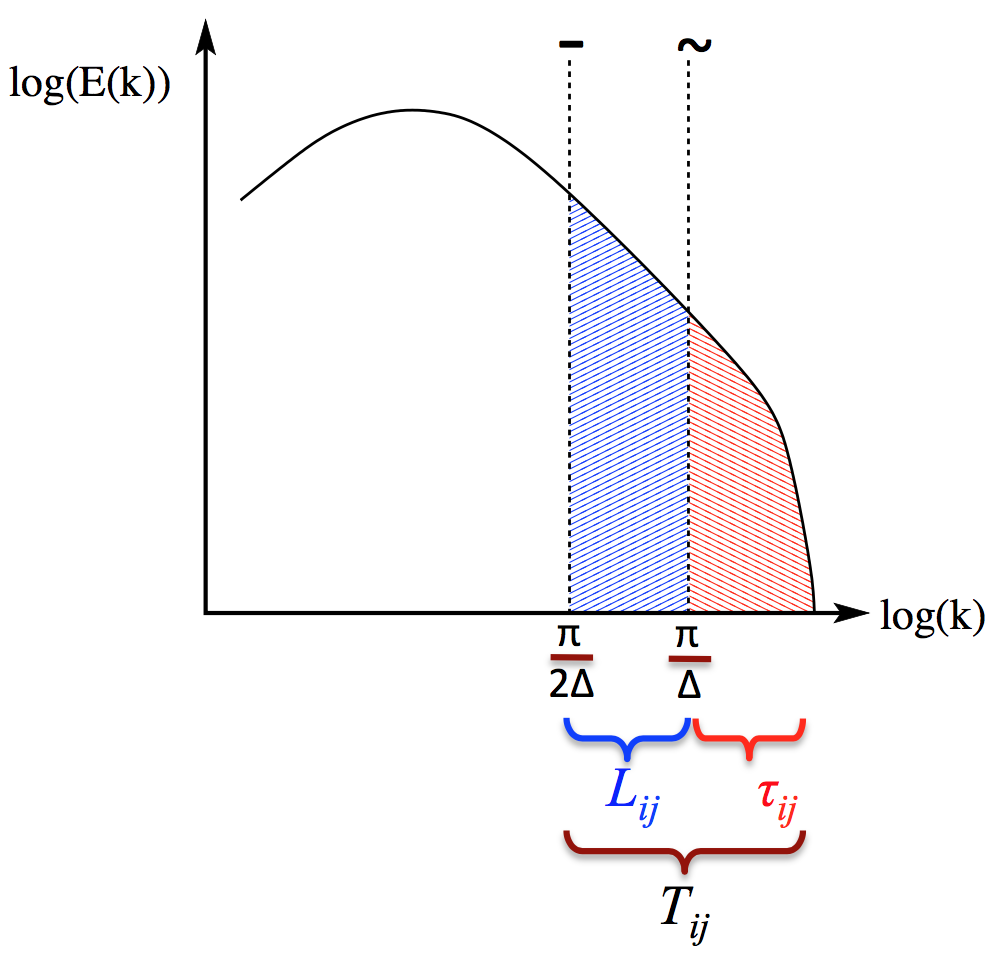
\includegraphics[width=0.55\textwidth]{germano1}
	\end{figure}
\end{itemize}
\end{frame}

%------------------------------------------------
\begin{frame}{Dynamic SGS Models}
\begin{itemize}
	\item Equation (\ref{sfs4}) is an identity -- \textbf{it is exact!} It can be exploited to derive model coefficients for common SGS models
	\item This identity is usually referred to as the \textbf{Germano identity}
	\item We will use the Smagorinsky model as an example of how one can use the Germano identity to find model coefficients. 
	\item Procedurally, we can follow the same steps (presented next) for any base SGS model
\end{itemize}
\end{frame}

%------------------------------------------------
\subsection{Dynamic Smagorinsky Model}
%------------------------------------------------
\begin{frame}{Dynamic Smagorinsky Model}
\begin{itemize}
	\item The first assumption we must make is that the same model (e.g. Smagorinsky model) can be applied for the stress at $\Delta$ and $\alpha \Delta$ (say, $2\Delta$)
	\item Using the Smagorinsky model in the Germano identity (Note Smagorinsky is only for anisotropic part)
	\begin{align*}
	L_{ij} - \frac{1}{3}\delta_{ij}L_{kk} &= T_{ij} - \overline{\tau_{ij}}\\
	\overline{\widetilde{u}_i\widetilde{u}_j} - \overline{\widetilde{u}_i}\;\overline{\widetilde{u}_j} &= -2(C_S \alpha \Delta)^2\left|\overline{\widetilde{S}}\right|\overline{\widetilde{S}}_{ij} + \overline{2(C_S\Delta)^2\left|\widetilde{S}\right|\widetilde{S}_{ij}}
	\end{align*}
\end{itemize}
\end{frame}

%------------------------------------------------
\begin{frame}{Dynamic Smagorinsky Model}
\begin{itemize}
	\item  For the next parts we will follow Lilly (1992)
	\item We can rearrange this equation to write an expression for the error associated with
using the Smagorinsky model in the Germano identity
	$$e_{ij} = L_{ij} - \frac{1}{3}\delta_{ij}L_{kk}-\left[-2(C_S \alpha \Delta)^2\left|\overline{\widetilde{S}}\right|\overline{\widetilde{S}}_{ij} + \overline{2(C_S\Delta)^2\left|\widetilde{S}\right|\widetilde{S}_{ij}}\right]$$
	\item This can be rewritten as (note: we assume $L_{ij}$ is trace free)
	$$e_{ij} = L_{ij} - C_S^2 M_{ij}$$
	where
	$$M_{ij} = 2\Delta^2\left[\overline{\left|\widetilde{S}\right|\widetilde{S}_{ij}} - \alpha^2\left|\overline{\widetilde{S}}\right|\overline{\widetilde{S}}_{ij}\right]$$
	\item Problem: This is 9 equations with only 1 unknown!
\end{itemize}
\end{frame}

%------------------------------------------------
\begin{frame}{Dynamic Smagorinsky Model}
\begin{itemize}
	\item  Lilly (1992) proposed to minimize the error in a least-squares sense. That is, we want the least-square error of using the Smagorinsky model in the Germano identity
	\item The squared error is
	$$e_{ij}^2 = (L_{ij} - C_S^2M_{ij})^2 = L_{ij}^2 - 2C_S^2 L_{ij}M_{ij} + (C_S^2)^2M_{ij}M_{ij}$$
	\item We want the minimum w.r.t. $C_S^2$ (\textit{i.e.}, $\partial e_{ij}^2/\partial C_S^2 = 0$)
	$$\frac{\partial e_{ij}^2}{\partial C_S^2} = -2L_{ij}M_{ij} + 2C_S^2M_{ij}M_{ij} = 0$$
	Solving for $C_S^2$ yields
	$$\boxed{C_S^2 = \frac{L_{ij}M_{ij}}{M_{ij}M_{ij}}}$$
\end{itemize}
\end{frame}

%------------------------------------------------
\begin{frame}{Dynamic Smagorinsky Model}
\begin{itemize}
	\item Problem: the above local form of the dynamic Smagorinsky coefficient is numerically unstable
	\item Remember that the instantaneously energy cascade can be forward or backwards 
	\item In simulations, this was found to lead to numerical instability (having $\pm C_S^2$)
	\item The instability is attributed to high time correlations of $C_S^2$ (\textit{i.e.}, when $C_S^2$ is negative at a point it tends to stay negative)
	\item Why do we have this problem? \textbf{We had to make 2 assumptions to derive the $C_S^2$ equation!}
\end{itemize}
\end{frame}

%------------------------------------------------
\subsection{Assumptions in the Dynamic Model}
%------------------------------------------------
\begin{frame}{Assumptions in the Dynamic Model}
\textbf{\nth{1} Assumption}
\begin{itemize}
	\item $C_S^2$ is constant over the filter width $\alpha\Delta$ (-- filter in the equations)
	\item Recall our basic definition of a convolution filter
	$$\tilde \phi (\vec{x},t) = \int_{-\infty}^{\infty} \phi (\vec{x} - \vec{\zeta},t) G(\vec{\zeta}) d \vec{\zeta}$$
	If we look at the error equations, we notice that $C_S^2$ falls under the bar filter
	$$e_{ij} = L_{ij} - \frac{1}{3}\delta_{ij}L_{kk}-\left[-2(C_S \alpha \Delta)^2\left|\overline{\widetilde{S}}\right|\overline{\widetilde{S}}_{ij} + \overline{2(C_S\Delta)^2\left|\widetilde{S}\right|\widetilde{S}_{ij}}\right]$$
	\item This is actually a \textbf{set of integral equations} if we don’t make our assumption!
\end{itemize}
\end{frame}

%------------------------------------------------
\begin{frame}{Assumptions in the Dynamic Model}
\textbf{\nth{1} Assumption}, continued
\begin{itemize}
	\item  Ghosal et al. (1995) solved this equation for $C_S^2$ everywhere using a variational method -- which is \textbf{very expensive and complex}
	\item The constant $C_S^2$ (w.r.t. the test filter) assumption contributes to the previously discussed numerical instability
	\item The typical method (instead of the Ghosal method) is to enforce the Germano identity in an average sense
	$$\boxed{C_S^2 = \frac{\langle L_{ij}M_{ij}\rangle}{\langle M_{ij}M_{ij}\rangle}}$$
\end{itemize}
\end{frame}

%------------------------------------------------
\begin{frame}{Assumptions in the Dynamic Model}
\textbf{\nth{1} Assumption}, continued
\begin{itemize}
	\item Constraining $C_S^2$ removes its oscillations -- resulting in stable simulations 
	\item Typically, the average is enforced over some region of spatial homogeneity
	\item For example in a homogeneous boundary layer over horizontal planes
	\item $\langle\ \rangle$ is an averaging operator, \textit{e.g.}, $C_S^2$ varies only in the wall normal direction
	\begin{figure}
		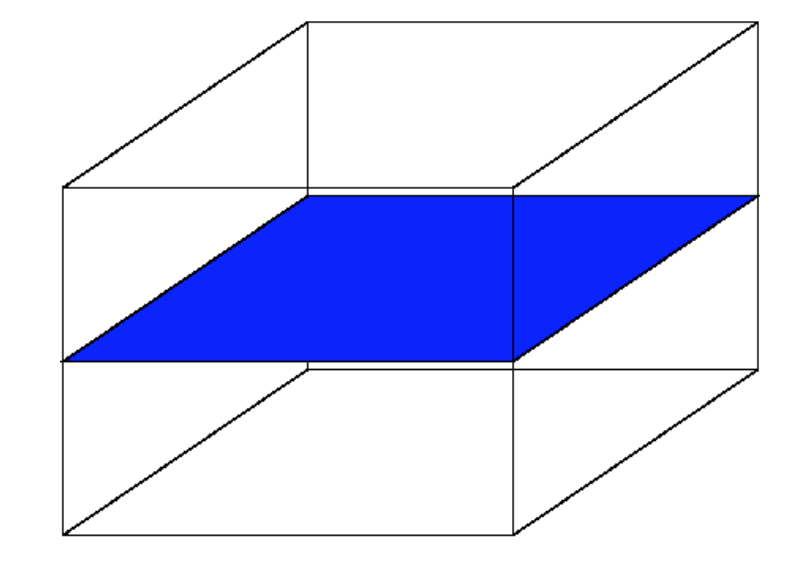
\includegraphics[width=0.5\textwidth]{germano2}
	\end{figure}
\end{itemize}
\end{frame}

%------------------------------------------------
\begin{frame}{Assumptions in the Dynamic Model}
\textbf{\nth{1} Assumption}, continued
\begin{itemize}
	\item Meneveau et al. (1996) developed the Lagrangian Dynamic model based on the idea that the Germano identity should be enforced along fluid particle trajectories
	\item Using \nth{1}-order time and space estimates, the average of any quantity $A$ (\textit{e.g.}, $L_{ij}$) can be defined as
	$$\langle A(\vec{x})\rangle^{n+1} = \gamma\left[A(\vec{x})\right]^{n+1} + (1-\gamma)\left[A(\vec{x}-\vec{u}^n\Delta t)\right]^n$$
	where $\gamma \equiv (\Delta t/T^n) / (1 + \Delta t/T^n)$ and $T$ is the Lagrangian timescale that controls how far back in time the average goes
	\begin{figure}
		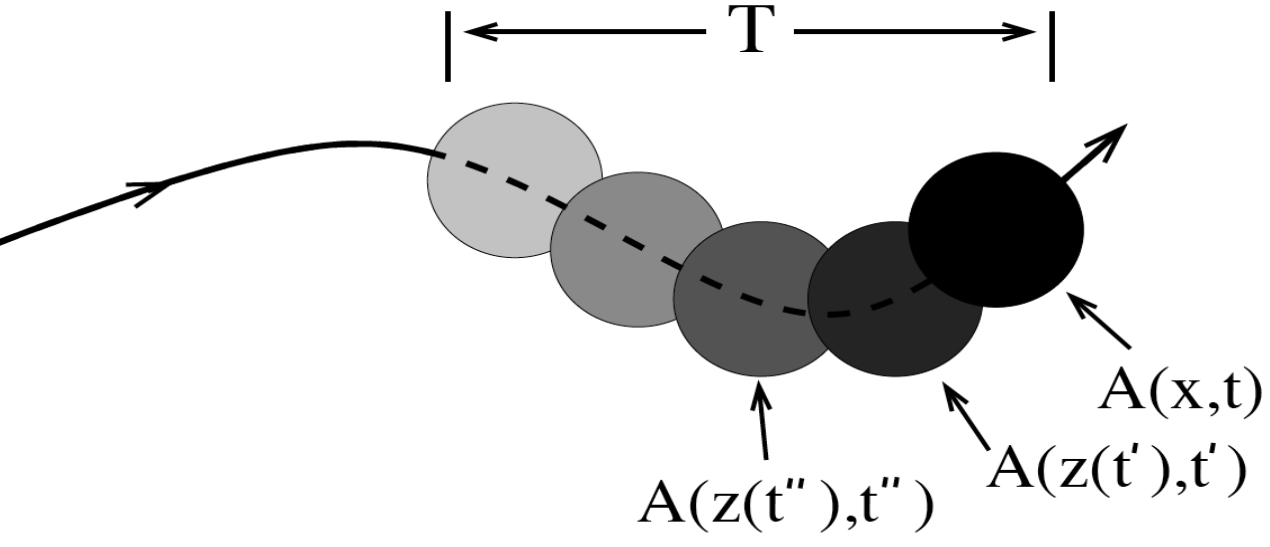
\includegraphics[width=0.5\textwidth]{germano3}
	\end{figure}
\end{itemize}
\end{frame}

%------------------------------------------------
\begin{frame}{Assumptions in the Dynamic Model}
\textbf{\nth{2} Assumption}
\begin{itemize}
	\item When we applied the Smagorinsky model to the Germano identity at 2 different scales, \textbf{we made the assumption that the same $C_S^2$ applies at both scales}
	\item \textit{i.e.}, we assumed $C_S^2(\Delta) = C_S^2(2\Delta)$, or in other words scale invariance of $C_S^2$
	\item  This assumption is not bad provided that both of our filter scales $\Delta$ and $2\Delta$ are in the inertial subrange of turbulence
	\item We will violate this assumption in some region of the flow (\textit{e.g.}, near the wall in a boundary layer when $z \leq 2\Delta$) for cases with at least 1 direction of flow anisotropy
\end{itemize}
\end{frame}

%------------------------------------------------
\begin{frame}{Assumptions in the Dynamic Model}
\textbf{\nth{2} Assumption}, continued
\begin{itemize}
	\item Port\'{e}-Agel et al., (2000) developed a generalized dynamic model where $C_S^2$ is a function of scale
	\item They made the weaker assumption that $C_S^2$ follows a power law distribution at the smallest resolved scales, \textit{e.g.}
	$$\frac{C_S^2(2\Delta)}{C_S^2(\Delta} = \frac{C_S^2(4\Delta)}{C_S^2(2\Delta}$$
\end{itemize}
\end{frame}

%------------------------------------------------
\begin{frame}{Assumptions in the Dynamic Model}
\textbf{\nth{2} Assumption}, continued
\begin{itemize}
	\item So now in our equation for $C_S^2$, we have
	$$M_{ij} = 2\Delta^2\left[\overline{\left|\widetilde{S}\right|\widetilde{S}_{ij}} - \alpha^2\beta\left|\overline{\widetilde{S}}\right|\overline{\widetilde{S}}_{ij}\right]$$
	where
	$$\beta = \frac{C_S^2(2\Delta)}{C_S^2(\Delta)}$$
	is the scale-dependence coefficient	
\end{itemize}
\end{frame}

%------------------------------------------------



\end{document}

